\documentclass[11pt]{article}
\usepackage[letterpaper,margin=1in]{geometry}
\usepackage{amsmath,amssymb,bm}
\usepackage{graphicx}
\usepackage{booktabs}
\usepackage{float}
\usepackage{caption}
\usepackage{subcaption}
\usepackage{enumitem}
\usepackage{tikz}
\usetikzlibrary{positioning,arrows.meta}
\usepackage[hidelinks]{hyperref}
\setlength{\parindent}{0pt}
\setlength{\parskip}{6pt}
\newcommand{\R}{\mathbb{R}}
\newcommand{\sm}{\sigma(\mathbf{z})}
\DeclareMathOperator{\diag}{diag}
\DeclareMathOperator{\ReLU}{ReLU}

\title{Homework 3: Building Your Neural Network\\[4pt]\large EN.705.641.81 Natural Language Processing: Self-Supervised Models}
\author{Brian Onieal}
\date{Module 4, Fall 2026}

\begin{document}
\maketitle

\textbf{Name:} Brian Onieal

\textbf{Collaborators, if any:} None

\textbf{Sources used for your homework, if any:} Claude (Anthropic), as described in the disclosure below. The PyTorch documentation linked in the assignment. The upstream JHU CS 601.471/671 hw3 skeleton, for the fixed hyper-parameters of the two experiment functions missing from the class template (Section 6.1.4). The papers cited inline.

\noindent\rule{0.6\textwidth}{0.4pt}

\textbf{GenAI Disclosure}
\begin{quote}
Claude (Anthropic, model \texttt{claude-opus-5-5}) was used to produce the written answers, derivations, and figures in this document, to complete the code in the accompanying repository, and to run the programming experiments and generate the plots in Section 6. The results that can be computed (the Jacobians in Section 2, the softmax Jacobian, the XOR networks in Section 4, and the computation graph in Section 5) were also checked numerically with PyTorch autograd, using the scripts in the repository's \texttt{verification/} folder. The three \texttt{Copy from your HW1} blocks in \texttt{mlp.py} (\texttt{featurize}, the \texttt{create\_tensor\_dataset} loop, and \texttt{accuracy}) are adapted from my Homework 1 submission. I directed the work and reviewed it before submitting. Code generated with Claude's assistance is identified in the header comment of each \texttt{.py} file.
\end{quote}
\noindent\rule{0.6\textwidth}{0.4pt}

%======================================================================
\section{Concepts, intuitions and big picture}

\subsection*{1.1 Zero initialization}
\textbf{Answer:} Only the first statement is true. Each neuron in the first hidden layer performs the same computation, and it keeps computing the same thing as the other neurons in its layer after any number of gradient descent iterations.

\textbf{Derivation.} Write hidden unit $j$ as $z_j = \mathbf{w}_j^\top \mathbf{x} + b_j$, $a_j = g(z_j)$, and let $W^{[2]}$ be the outgoing weights. With every weight and bias at zero:
\begin{align*}
z_j &= \mathbf{0}^\top\mathbf{x} + 0 = 0 \quad\text{for every } j, \qquad a_j = g(0) \quad\text{for every } j.
\end{align*}
Backpropagation gives, for unit $j$,
\begin{align*}
\delta_j = \frac{\partial L}{\partial z_j} = \Big(\sum_k W^{[2]}_{kj}\,\delta^{[2]}_k\Big)\, g'(z_j),
\qquad
\frac{\partial L}{\partial \mathbf{w}_j} = \delta_j\,\mathbf{x}^\top,
\qquad
\frac{\partial L}{\partial W^{[2]}_{kj}} = \delta^{[2]}_k\, a_j .
\end{align*}
Column $j$ of $W^{[2]}$ is the same for every $j$ (all zeros) and $z_j$ is the same for every $j$, so $\delta_j$ is the same for every $j$. Every row $\mathbf{w}_j$ therefore receives the same update. Every column of $W^{[2]}$ also receives the same update, because $a_j$ is the same for every $j$. By induction on the step number, if the rows of $W^{[1]}$ and the columns of $W^{[2]}$ are identical before a step, they are identical after it. (For zero initialization in particular, $W^{[2]}=0$ makes $\delta_j = 0$ on the first step, so the first layer does not move at all.)

Why the other three are false. Statement 2: the updates are identical, so one step of gradient descent cannot break the tie. Statement 3: different layers computing different things does not help, because within each layer every unit is still a copy of one unit. Statement 4: in the first iteration $z_j = 0$ for all $j$, so they do not compute different things.

\subsection*{1.2 Vectorization across layers}
\textbf{Answer: False.} Layer $l$ computes $A^{[l]} = g\big(W^{[l]}A^{[l-1]} + \mathbf{b}^{[l]}\big)$, which needs $A^{[l-1]}$ as input. That dependence forces the layers to be computed in order $l = 1, 2, \dots, L$, so an explicit loop over layers remains. Vectorization removes the loop over the examples in a batch (they are the columns of $A^{[l-1]}$) and the loop over units inside a layer (one matrix product), not the loop over layers.

\subsection*{1.3 Tanh versus sigmoid}
\textbf{Answer: True.} The two functions are related by
\[
\tanh(x) = \frac{e^{x}-e^{-x}}{e^{x}+e^{-x}} = \frac{1-e^{-2x}}{1+e^{-2x}} = \frac{2}{1+e^{-2x}} - 1 = 2\sigma(2x) - 1 .
\]
So tanh is a sigmoid rescaled to the range $(-1,1)$ and centered so that $\tanh(0)=0$, while $\sigma(0)=0.5$ and $\sigma(x)\in(0,1)$. Hidden activations that average near zero give the next layer centered inputs, which is better for its gradient updates (derivation in 3.4). Tanh also has a larger slope at the origin, $\tanh'(0)=1$ versus $\sigma'(0)=1/4$.

\subsection*{1.4 Which technique does NOT prevent overfitting?}
\textbf{Answer: None of the above.} All three reduce overfitting. Data augmentation adds label-preserving variations of the training examples, which gives the model more data and lowers variance. Dropout randomly zeroes units during training, which acts as a regularizer (1.5). Early stopping halts training when dev loss stops improving, which limits how far the weights can move toward fitting noise in the training set.

\subsection*{1.5 Dropout at training time and not at evaluation time}
With drop probability $p$, inverted dropout (what \texttt{nn.Dropout} does) replaces each activation $h_i$ during training with
\[
\tilde h_i = \frac{m_i\,h_i}{1-p}, \qquad m_i \sim \text{Bernoulli}(1-p).
\]
\textbf{Why apply it during training.} A unit cannot rely on any particular other unit being present, so units cannot co-adapt into fragile combinations that only fit the training set. Each mini-batch trains a different thinned sub-network, so the full network behaves like an ensemble of up to $2^N$ weight-sharing sub-networks for $N$ droppable units, and averaging an ensemble reduces variance. The $1/(1-p)$ scaling keeps the expected activation unchanged:
\[
\mathbb{E}[\tilde h_i] = (1-p)\cdot\frac{h_i}{1-p} + p\cdot 0 = h_i,
\qquad
\operatorname{Var}[\tilde h_i] = h_i^2\,\frac{p}{1-p} > 0 .
\]
\textbf{Why not apply it during evaluation.} At evaluation we want the ensemble's averaged prediction, and we want it to be deterministic. Averaging over all $2^N$ masks exactly is intractable, but using every unit with its expected activation approximates that average, and the expectation above shows the training-time scaling already makes the plain activation $h_i$ the right value to use. Keeping dropout on at evaluation would inject the variance $h_i^2\,p/(1-p)$ into every prediction, so the same input could get different outputs and accuracy would drop. In PyTorch, \texttt{model.eval()} turns \texttt{nn.Dropout} into the identity and \texttt{model.train()} turns it back on. The skeleton's language model training loop in \texttt{mlp\_lm.py} calls \texttt{evaluate()}, which switches to eval mode, and never switches back, so I added \texttt{model.train()} at the start of each epoch. Without it, dropout would be off from the second epoch on.

\subsection*{1.6 Initializing with a constant}
Suppose every weight in a layer equals the same constant $c$ (and the biases share a value $\beta$). Then every unit in that layer sees the same pre-activation and outputs the same value:
\[
z_j = c\sum_k x_k + \beta \quad\text{for all } j \;\Longrightarrow\; a_j = g(z_j) \text{ is the same for all } j.
\]
The backward pass gives $\partial L/\partial W_{jk} = \delta_j x_k$ with $\delta_j = \big(\sum_m W^{\text{next}}_{mj}\delta^{\text{next}}_m\big)\,g'(z_j)$. The outgoing weights $W^{\text{next}}_{:,j}$ are also constant, so $\delta_j$ is the same for every $j$ and every unit gets the same update. The units start identical and, by the same induction as 1.1, stay identical for the whole run. A layer of $n$ units then has the capacity of a single unit, and the network wastes almost all of its parameters. This is the symmetry problem, and random initialization is what breaks it. The numerical check for the XOR network in 4.4 shows it: after 20{,}000 gradient descent steps from a constant initialization, the two hidden units still had identical weights. A constant of $c = 0$ is the worst case, because it also zeroes the gradient reaching earlier layers (4.3). A large constant has a second problem, saturation, covered next.

\subsection*{1.7 All-sigmoid network initialized with large positive weights}
\textbf{Answer: No, it is a bad idea.} With large positive weights, pre-activations $z = W\mathbf{a} + \mathbf{b}$ are large. Every sigmoid output is positive, so after the first layer all inputs to a unit are positive and all its weights are positive, and every term in $z_j = \sum_k W_{jk}a_k$ adds in the same direction. The units saturate at $\sigma(z)\approx 1$, where the slope vanishes:
\[
\sigma'(z) = \sigma(z)\big(1-\sigma(z)\big), \qquad \sigma'(5) \approx 6.6\times10^{-3}, \qquad \sigma'(10) \approx 4.5\times10^{-5}.
\]
Backpropagation multiplies by this slope at every layer, $\boldsymbol\delta^{[l]} = \big(W^{[l+1]\top}\boldsymbol\delta^{[l+1]}\big)\odot\sigma'(\mathbf{z}^{[l]})$, so the gradient shrinks toward zero and learning stalls (the vanishing gradient problem of 3.3). Larger weights do not rescue it. For $u>0$, $\sigma'(u) = \dfrac{e^{-u}}{(1+e^{-u})^2} \le e^{-u}$ because the denominator is at least $1$. So for one unit with input $s > 0$ and weight $w>0$, the factor passed back satisfies $0 < w\,\sigma'(ws) \le w\,e^{-ws}$, which goes to $0$ as $w\to\infty$ because the exponential wins over the linear term. The forward pass is damaged too: a saturated unit outputs about $1$ for nearly every input, so it carries almost no information about $\mathbf{x}$ to the next layer. Small random weights (for example Xavier initialization, $\operatorname{Var}(W_{jk}) = 2/(n_{\text{in}}+n_{\text{out}})$) keep $z$ in the region where $\sigma'$ is close to its maximum of $1/4$.

\subsection*{1.8 Why residual connections matter}
A residual block adds its input back to its output, $\mathbf{x}_{l+1} = \mathbf{x}_l + F_l(\mathbf{x}_l)$. Its Jacobian is
\[
\frac{\partial \mathbf{x}_{l+1}}{\partial \mathbf{x}_l} = I + \frac{\partial F_l}{\partial \mathbf{x}_l},
\]
so the gradient reaching layer $l$ from the output of an $L$-layer stack is
\[
\frac{\partial \mathcal{L}}{\partial \mathbf{x}_l} = \frac{\partial \mathcal{L}}{\partial \mathbf{x}_L}\prod_{i=L-1}^{l}\Big(I + \frac{\partial F_i}{\partial \mathbf{x}_i}\Big)
= \frac{\partial \mathcal{L}}{\partial \mathbf{x}_L}\Big(I + \sum_{i}\frac{\partial F_i}{\partial \mathbf{x}_i} + \cdots\Big).
\]
The leading $I$ term delivers the loss gradient to every layer unchanged, even when the individual $\partial F_i/\partial\mathbf{x}_i$ are small. Without the skip path the gradient is the bare product $\prod_i \partial F_i/\partial \mathbf{x}_i$, which shrinks or grows exponentially with depth. Residual connections matter for three reasons. They keep gradients flowing through very deep networks. They make the identity map easy to learn (drive $F_l$ to zero), so adding a layer should not make the best achievable training loss worse, and each layer only has to learn a correction to its input. And they are what made networks with 100+ layers trainable (He et al., 2016, \emph{Deep Residual Learning for Image Recognition}, CVPR). Every Transformer block uses them. In this homework, \texttt{NPLMBlock} in \texttt{mlp\_lm.py} is a residual block, \texttt{hidden = inputs + tanh(linear(inputs))}.

\subsection*{1.9 What is cached}
\textbf{Answer:} The first option. Variables computed during forward propagation are cached and passed to the corresponding backward step to compute derivatives. For layer $l$ the backward step needs values from the forward step:
\[
d Z^{[l]} = dA^{[l]}\odot g'\big(Z^{[l]}\big), \qquad dW^{[l]} = \tfrac{1}{m}\,dZ^{[l]}A^{[l-1]\top}, \qquad dA^{[l-1]} = W^{[l]\top}dZ^{[l]},
\]
so $Z^{[l]}$, $A^{[l-1]}$, and $W^{[l]}$ are cached. The second option describes hyper-parameter search, which has nothing to do with caching, and the third reverses the direction of the data flow.

\subsection*{1.10 Deeper versus earlier layers}
\textbf{Answer:} The first statement. Deeper layers typically compute more complex features, because each layer builds its features out of the features computed by the layer below, so depth composes simple functions into more complex ones. In vision, early layers respond to edges and later ones to parts and objects. In NLP, probing studies of BERT find lower layers encode more surface and syntactic information and higher layers more semantic information (Jawahar et al., 2019, \emph{What Does BERT Learn about the Structure of Language?}, ACL, and Tenney et al., 2019, \emph{BERT Rediscovers the Classical NLP Pipeline}, ACL).

%======================================================================
\section{Revisiting Jacobians}
Conventions. $\mathbf{w}\in\R^{d\times 1}$. The Jacobian has shape (shape of output) $\times$ (shape of input), with entry $\partial f_a/\partial w_b$ in row $a$, column $b$. A scalar output therefore gives a $1\times d$ row vector. Every result below was checked against \texttt{torch.autograd.functional.jacobian} on random inputs (\texttt{verification/verify\_theory.py}).

\subsection*{2.1 $f(\mathbf{w}) = c$}
Shape $1\times d$. For every $j$, $\partial c/\partial w_j = 0$. So $\mathbf{J} = \mathbf{0}^\top = [0\ \cdots\ 0] \in \R^{1\times d}$.

\subsection*{2.2 $f(\mathbf{w}) = \|\mathbf{w}\|^2$}
Shape $1\times d$. Write $f = \mathbf{w}^\top\mathbf{w} = \sum_{i=1}^d w_i^2$. Then
\[
\frac{\partial f}{\partial w_j} = \sum_{i=1}^d 2w_i\,\frac{\partial w_i}{\partial w_j} = \sum_{i=1}^d 2w_i\,\delta_{ij} = 2w_j,
\qquad
\mathbf{J} = [2w_1\ \cdots\ 2w_d] = 2\mathbf{w}^\top \in\R^{1\times d}.
\]

\subsection*{2.3 $f(\mathbf{w}) = \mathbf{w}^\top\mathbf{x}_i$}
Shape $1\times d$. Write $f = \sum_{j=1}^d w_j x_{ij}$, where $x_{ij}$ is entry $j$ of $\mathbf{x}_i$. Then
\[
\frac{\partial f}{\partial w_j} = x_{ij}, \qquad \mathbf{J} = [x_{i1}\ \cdots\ x_{id}] = \mathbf{x}_i^\top\in\R^{1\times d}.
\]

\subsection*{2.4 $f(\mathbf{w}) = X\mathbf{w}$}
The output is $n\times 1$, so the shape is $n\times d$. Entry $a$ of the output is $f_a = \sum_{j=1}^d X_{aj}w_j$, so
\[
\frac{\partial f_a}{\partial w_b} = \sum_{j=1}^d X_{aj}\,\delta_{jb} = X_{ab}, \qquad \mathbf{J} = X\in\R^{n\times d}.
\]
Row $a$ of $\mathbf{J}$ is $\mathbf{x}_a^\top$, which matches 2.3 applied to each row of $X$.

\subsection*{2.5 $f(\mathbf{w}) = \mathbf{w}$}
Shape $d\times d$. $f_a = w_a$, so $\partial f_a/\partial w_b = \delta_{ab}$ and $\mathbf{J} = I_d\in\R^{d\times d}$.

\subsection*{2.6 $f(\mathbf{w}) = \mathbf{w}^2$ (element-wise)}
Shape $d\times d$. $f_a = w_a^2$ depends only on $w_a$, so
\[
\frac{\partial f_a}{\partial w_b} = 2w_a\,\delta_{ab}, \qquad
\mathbf{J} = \diag(2\mathbf{w}) = \begin{bmatrix} 2w_1 & & 0\\ & \ddots & \\ 0 & & 2w_d\end{bmatrix}\in\R^{d\times d}.
\]
Any element-wise function gives a diagonal Jacobian, because output $a$ depends on input $a$ alone.

\subsection*{2.7 Extra credit: $F(W) = XW^\top$}
Shapes: $X\in\R^{n\times d}$, $W\in\R^{k\times d}$, so $W^\top\in\R^{d\times k}$ and $F\in\R^{n\times k}$. The Jacobian has shape (output) $\times$ (input) $= (n\times k)\times(k\times d)$, a 4th-order tensor with $nk\cdot kd$ entries.

Entry $(a,b)$ of the output is the dot product of row $a$ of $X$ with row $b$ of $W$:
\[
F_{ab} = \sum_{c=1}^{d} X_{ac}\,(W^\top)_{cb} = \sum_{c=1}^{d} X_{ac}W_{bc} = \mathbf{x}_a^\top\mathbf{w}_b .
\]
Differentiate with respect to the input entry $W_{pq}$, using $\partial W_{bc}/\partial W_{pq} = \delta_{bp}\delta_{cq}$:
\[
\mathbf{J}_{ab,pq} = \frac{\partial F_{ab}}{\partial W_{pq}} = \sum_{c=1}^d X_{ac}\,\delta_{bp}\,\delta_{cq} = \delta_{bp}\,X_{aq}.
\]
So output $(a,b)$ depends only on row $b$ of $W$, and its gradient with respect to that row is $\mathbf{x}_a^\top$: $\partial F_{ab}/\partial W = \mathbf{e}_b\mathbf{x}_a^\top\in\R^{k\times d}$, a matrix that is zero except for row $b$. The same Jacobian can be written as a matrix. Flatten $F$ row by row, so $F_{ab}$ sits at position $(a-1)k+b$, and flatten $W$ column by column, so $W_{pq}$ sits at position $(q-1)k+p$ (this pairing is the one that gives a clean Kronecker form). The Kronecker product $X\otimes I_k$ has entry $(X\otimes I_k)_{(a-1)k+b,\,(q-1)k+p} = X_{aq}\,(I_k)_{bp} = X_{aq}\,\delta_{bp}$, which is $\mathbf{J}_{ab,pq}$. So the flattened Jacobian is the $nk\times kd$ matrix $X\otimes I_k$. Both forms match autograd.

%======================================================================
\section{Activations Per Layer, Keeps Linearity Away!}

\subsection*{3.1 Why activation functions are used}
Without a non-linearity, stacking layers gains nothing, because a composition of affine maps is affine:
\[
\mathbf{h}^{[2]} = W_2\big(W_1\mathbf{x}+\mathbf{b}_1\big)+\mathbf{b}_2 = \underbrace{(W_2W_1)}_{W'}\mathbf{x} + \underbrace{(W_2\mathbf{b}_1+\mathbf{b}_2)}_{\mathbf{b}'} .
\]
By induction, any number of linear layers equals one linear layer $W'\mathbf{x}+\mathbf{b}'$, whose decision boundaries are hyperplanes. Such a model cannot represent XOR (4.1). Putting a non-linear function between the layers stops the collapse. With a non-polynomial activation such as sigmoid, tanh, or ReLU, a network with even one hidden layer of enough units can approximate any continuous function on a compact set to any accuracy (Cybenko, 1989, \emph{Approximation by Superpositions of a Sigmoidal Function}. Hornik, 1991, \emph{Approximation Capabilities of Multilayer Feedforward Networks}. Leshno et al., 1993, \emph{Multilayer Feedforward Networks with a Nonpolynomial Activation Function Can Approximate Any Function}). Activation functions are what let depth add expressive power.

\subsection*{3.2 Sigmoid, ReLU, and tanh with their derivatives}
\textbf{Sigmoid.} $\sigma(x) = \dfrac{1}{1+e^{-x}}$, range $(0,1)$, with $\sigma(x)\to 0$ as $x\to-\infty$ and $\sigma(x)\to 1$ as $x\to+\infty$.
\[
\sigma'(x) = \frac{d}{dx}\big(1+e^{-x}\big)^{-1} = -\big(1+e^{-x}\big)^{-2}\cdot\big(-e^{-x}\big) = \frac{1}{1+e^{-x}}\cdot\frac{e^{-x}}{1+e^{-x}} = \sigma(x)\big(1-\sigma(x)\big),
\]
using $1-\sigma(x) = e^{-x}/(1+e^{-x})$. Its maximum is $\sigma'(0) = \tfrac12\cdot\tfrac12 = \tfrac14$, and $\sigma'(x)\to 0$ as $|x|\to\infty$.

\textbf{ReLU.} $\ReLU(x) = \max(0,x)$, range $[0,\infty)$.
\[
\ReLU'(x) = \begin{cases} 1, & x>0\\ 0, & x<0\end{cases}
\]
At $x=0$ the left derivative is $0$ and the right derivative is $1$, so the derivative is undefined there. PyTorch uses the subgradient value $0$ at $x=0$.

\textbf{Tanh.} $\tanh(x) = \dfrac{e^{x}-e^{-x}}{e^{x}+e^{-x}}$, range $(-1,1)$. By the quotient rule, with $u = e^x - e^{-x}$ and $v = e^x + e^{-x}$ (so $u' = v$ and $v' = u$):
\[
\tanh'(x) = \frac{u'v - uv'}{v^2} = \frac{v^2-u^2}{v^2} = 1-\frac{u^2}{v^2} = 1-\tanh^2(x).
\]
Its maximum is $\tanh'(0) = 1$, and $\tanh'(x)\to 0$ as $|x|\to\infty$.

Figure~\ref{fig:act} plots each function (solid) and its derivative (dashed). The plot window is $[-6,6]$. Past that range on both sides, sigmoid and tanh sit on their asymptotes with derivatives indistinguishable from $0$, and ReLU continues as $0$ on the left and the line $y=x$ on the right.

\begin{figure}[H]
\centering
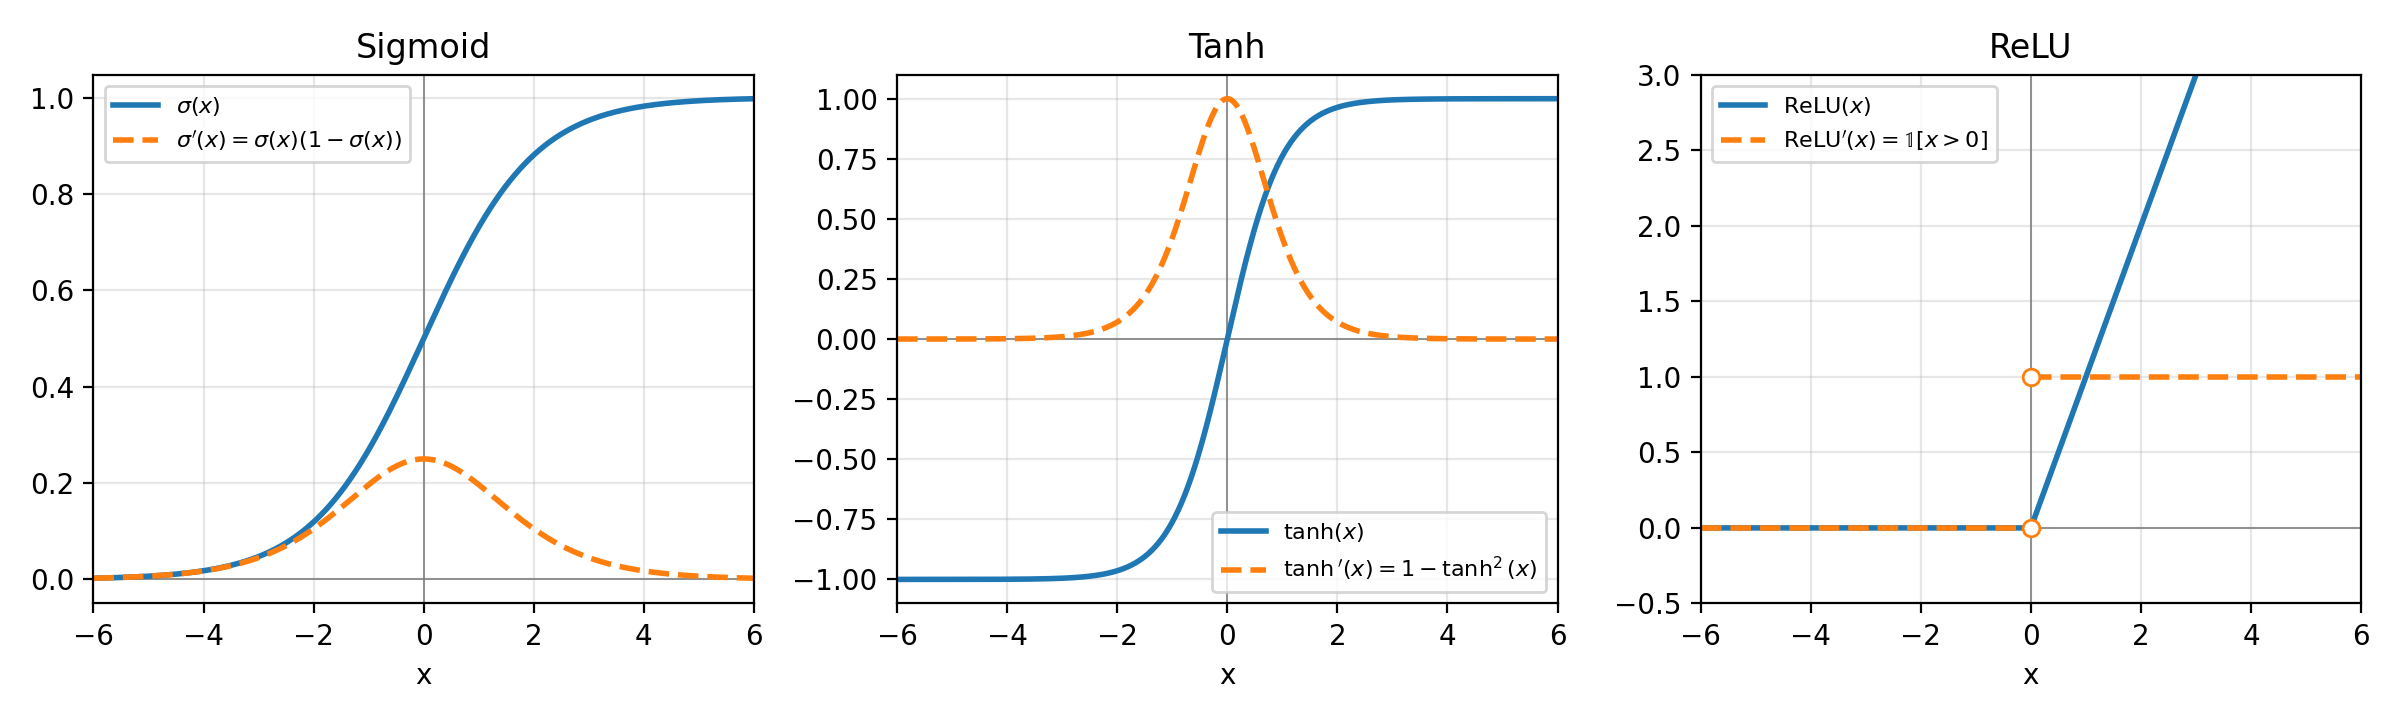
\includegraphics[width=\textwidth]{fig/activations.png}
\caption{Sigmoid, tanh, and ReLU (solid) and their derivatives (dashed). The open circles on the ReLU derivative mark the jump at $x=0$, where the derivative is undefined.}
\label{fig:act}
\end{figure}

\subsection*{3.3 The vanishing gradient problem}
\textbf{What it is.} Backpropagation computes the gradient at layer $l$ as a product of one Jacobian per layer above it, $\frac{\partial \mathcal{L}}{\partial \mathbf{h}^{[l]}} = \frac{\partial \mathcal{L}}{\partial \mathbf{h}^{[L]}}\,J^{[L]}J^{[L-1]}\cdots J^{[l+1]}$, where the chain rule applied to $\mathbf{h}^{[i]} = g(\mathbf{z}^{[i]})$ with $\mathbf{z}^{[i]} = W^{[i]}\mathbf{h}^{[i-1]}+\mathbf{b}^{[i]}$ gives $J^{[i]} = \frac{\partial\mathbf{h}^{[i]}}{\partial\mathbf{z}^{[i]}}\frac{\partial\mathbf{z}^{[i]}}{\partial\mathbf{h}^{[i-1]}} = \diag\big(g'(\mathbf{z}^{[i]})\big)W^{[i]}$. When those factors have norm below 1, the product shrinks exponentially with depth, so the early layers get almost no gradient and barely learn. It hits deep feedforward networks and RNNs unrolled over long sequences, where the same recurrent weight matrix enters the product once per time step.

\textbf{Which activations and why.} Sigmoid and tanh are subject to it because they saturate: $\sigma'(x)\le 1/4$ and $\tanh'(x)\le 1$, and both derivatives go to $0$ as $|x|$ grows (3.2). With sigmoid each layer multiplies the gradient by at most $1/4$, so ten layers scale it by at most $(1/4)^{10}\approx 9.5\times 10^{-7}$ before the weights are even counted. ReLU's derivative is $1$ for every positive input, so it does not shrink the gradient through active units (inactive units pass back a zero gradient, which is the separate ``dying ReLU'' problem).

\subsection*{3.4 Why zero-centered activations matter for backprop}
Take one unit in the next layer, $z = \sum_i w_i a_i + b$, with upstream gradient $\delta = \partial\mathcal{L}/\partial z$. Its weight gradient is
\[
\frac{\partial\mathcal{L}}{\partial w_i} = \delta\, a_i \qquad\text{for every } i.
\]
If the incoming activations are all positive, as sigmoid outputs in $(0,1)$ always are, then every component of $\nabla_{\mathbf{w}}\mathcal{L}$ has the sign of the single scalar $\delta$. For one example, all of the unit's weights go up together or all go down together. If the better weight vector needs some weights to rise and others to fall, gradient descent can only get there by zig-zagging between the all-positive and all-negative directions, which slows convergence. Over a mini-batch the $\delta$'s of different examples can differ in sign, so the constraint is softer, but the same bias remains. Zero-centered activations such as tanh give $a_i$ of both signs, so the gradient components can have different signs and point more directly at the optimum. A non-zero mean in the activations also shifts the next layer's pre-activations by $\sum_i w_i\,\mathbb{E}[a_i]$, pushing units toward saturation. LeCun et al. (1998, \emph{Efficient BackProp}) recommend zero-mean inputs to every layer for these reasons, and batch and layer normalization re-center activations for the same reason.

\subsection*{3.5 Derivative of softmax}
Let $\sigma(\mathbf{z})_i = e^{z_i}/S$ with $S = \sum_{k=1}^K e^{z_k}$, and note $\partial S/\partial z_j = e^{z_j}$ and $\partial e^{z_i}/\partial z_j = \delta_{ij}e^{z_i}$. By the quotient rule,
\begin{align*}
\frac{\partial\sigma(\mathbf{z})_i}{\partial z_j}
&= \frac{\dfrac{\partial e^{z_i}}{\partial z_j}\,S - e^{z_i}\,\dfrac{\partial S}{\partial z_j}}{S^2}
= \frac{\delta_{ij}e^{z_i}S - e^{z_i}e^{z_j}}{S^2}
= \delta_{ij}\frac{e^{z_i}}{S} - \frac{e^{z_i}}{S}\cdot\frac{e^{z_j}}{S}\\[4pt]
&= \delta_{ij}\,\sigma(\mathbf{z})_i - \sigma(\mathbf{z})_i\,\sigma(\mathbf{z})_j
= \sigma(\mathbf{z})_i\big(\delta_{ij} - \sigma(\mathbf{z})_j\big). \qquad\blacksquare
\end{align*}
The two cases are $\partial\sigma_i/\partial z_i = \sigma_i(1-\sigma_i)$, which matches the sigmoid derivative of 3.2 as it should, and $\partial\sigma_i/\partial z_j = -\sigma_i\sigma_j$ for $i\ne j$.

\subsection*{3.6 Jacobian of softmax}
By 3.5, entry $(i,j)$ of $\mathbf{J}_\sigma(\mathbf{z})\in\R^{K\times K}$ is
\[
[\mathbf{J}_\sigma(\mathbf{z})]_{ij} = \frac{\partial\sigma(\mathbf{z})_i}{\partial z_j} = \sigma(\mathbf{z})_i\,\delta_{ij} - \sigma(\mathbf{z})_i\,\sigma(\mathbf{z})_j .
\]
The first term is $\sigma(\mathbf{z})_i$ when $i=j$ and $0$ otherwise, which is entry $(i,j)$ of $\diag(\sigma(\mathbf{z}))$. The second term is entry $(i,j)$ of the outer product of the column vector $\sigma(\mathbf{z})\in\R^{K\times1}$ with itself, $[\sigma(\mathbf{z})\sigma(\mathbf{z})^\top]_{ij} = \sigma(\mathbf{z})_i\,\sigma(\mathbf{z})_j$. Since the two matrices agree entry by entry,
\[
\mathbf{J}_\sigma(\mathbf{z}) = \diag\big(\sigma(\mathbf{z})\big) - \sigma(\mathbf{z})\,\sigma(\mathbf{z})^\top\in\R^{K\times K}. \qquad\blacksquare
\]
Two checks. The matrix is symmetric. Each row sums to zero, $\sum_j[\mathbf{J}]_{ij} = \sigma_i - \sigma_i\sum_j\sigma_j = 0$, which it must, because adding the same constant to every $z_j$ leaves softmax unchanged. A consequence used in every classifier in this course: for cross-entropy $\mathcal{L} = -\sum_i y_i\log\sigma_i$ with one-hot $\mathbf{y}$, $\partial\mathcal{L}/\partial z_j = -\sum_i \frac{y_i}{\sigma_i}\sigma_i(\delta_{ij}-\sigma_j) = -y_j + \sigma_j\sum_i y_i = \sigma_j - y_j$.

%======================================================================
\section{Simulating XOR}

\subsection*{4.1 A single-layer network cannot represent XOR}
\textbf{Answer: No.} Write $\hat y = \ReLU(t(\mathbf{x}))$ with $t(\mathbf{x}) = w_1x_1 + w_2x_2 + b$. At the four inputs,
\[
t_{00} = b,\qquad t_{01} = w_2+b,\qquad t_{10} = w_1+b,\qquad t_{11} = w_1+w_2+b,
\]
and these always satisfy the identity
\[
t_{01} + t_{10} = w_1+w_2+2b = t_{00} + t_{11}. \tag{$\ast$}
\]
XOR needs $\hat y = 1$ at $(0,1)$ and $(1,0)$, and $\ReLU(t)=1$ forces $t=1$, so $t_{01} = t_{10} = 1$ and the left side of $(\ast)$ is $2$. XOR needs $\hat y = 0$ at $(0,0)$ and $(1,1)$, and $\ReLU(t)=0$ forces $t\le 0$, so the right side of $(\ast)$ is at most $0$. Since $2 \not\le 0$, no $W$ and $b$ exist.

The same holds if we only ask the network to score the positive inputs higher than the negative ones (for example, predict 1 when $\hat y > 0.5$). ReLU is non-decreasing, so $\hat y_{01} > \hat y_{00}$ requires $t_{01} > t_{00}$, and likewise $t_{01} > t_{11}$, $t_{10} > t_{00}$, $t_{10} > t_{11}$. Adding the first and last gives $t_{01}+t_{10} > t_{00}+t_{11}$, which contradicts $(\ast)$. Geometrically, the inputs with $\hat y > 0$ form the half-plane $\mathbf{w}^\top\mathbf{x}+b>0$, and no line separates $\{(0,1),(1,0)\}$ from $\{(0,0),(1,1)\}$. This is the limitation of single-layer perceptrons that Minsky and Papert pointed out in \emph{Perceptrons} (1969).

\subsection*{4.2 A two-layer network that computes XOR}
\[
W_1 = \begin{bmatrix}1 & 1\\ 1 & 1\end{bmatrix},\qquad
\mathbf{b}_1 = \begin{bmatrix}0\\ -1\end{bmatrix},\qquad
W_2 = \begin{bmatrix}1 & -2\end{bmatrix},\qquad
b_2 = 0 .
\]
Check on all four inputs, with $\mathbf{z} = W_1\mathbf{x}+\mathbf{b}_1 = (x_1+x_2,\ x_1+x_2-1)^\top$:
\begin{center}\small
\begin{tabular}{cccccc}
\toprule
$\mathbf{x}$ & $\mathbf{z} = W_1\mathbf{x}+\mathbf{b}_1$ & $\mathbf{h} = \ReLU(\mathbf{z})$ & $\hat y = h_1 - 2h_2 + 0$ & XOR \\
\midrule
$(0,0)$ & $(0,\,-1)$ & $(0,\,0)$ & $0 - 0 = 0$ & 0\\
$(0,1)$ & $(1,\,0)$ & $(1,\,0)$ & $1 - 0 = 1$ & 1\\
$(1,0)$ & $(1,\,0)$ & $(1,\,0)$ & $1 - 0 = 1$ & 1\\
$(1,1)$ & $(2,\,1)$ & $(2,\,1)$ & $2 - 2 = 0$ & 0\\
\bottomrule
\end{tabular}
\end{center}
The first hidden unit counts how many inputs are 1. The second fires only when both are 1. The output subtracts twice the second from the first, which cancels the double count at $(1,1)$. This is the solution given in Goodfellow, Bengio, and Courville (2016, \emph{Deep Learning}, Section 6.1), and the hidden layer is what maps the four points into a space where a linear output layer can separate them.

\subsection*{4.3 Zero initialization never learns XOR}
Let the hidden layer have $H$ units, and start from $W_1 = 0\in\R^{H\times2}$, $\mathbf{b}_1 = \mathbf{0}$, $W_2 = 0\in\R^{1\times H}$, $b_2 = 0$. Write $g_n = \partial\ell(\hat y_n, y_n)/\partial\hat y_n$ for training example $n$, which exists because $\ell$ is differentiable.

\textbf{Forward pass}, for every input $\mathbf{x}$:
\[
\mathbf{z} = W_1\mathbf{x}+\mathbf{b}_1 = \mathbf{0},\qquad \mathbf{h} = \ReLU(\mathbf{0}) = \mathbf{0},\qquad \hat y = W_2\mathbf{h}+b_2 = b_2 .
\]
\textbf{Backward pass}, for one example (chain rule from the output down):
\begin{align*}
\frac{\partial\ell}{\partial b_2} &= g_n, &
\frac{\partial\ell}{\partial W_2} &= g_n\,\mathbf{h}^\top = \mathbf{0}^\top \ \ (\text{since } \mathbf{h}=\mathbf{0}),\\
\frac{\partial\ell}{\partial \mathbf{h}} &= W_2^\top g_n = \mathbf{0} \ \ (\text{since } W_2 = 0), &
\frac{\partial\ell}{\partial \mathbf{z}} &= \frac{\partial\ell}{\partial \mathbf{h}}\odot\ReLU'(\mathbf{z}) = \mathbf{0},\\
\frac{\partial\ell}{\partial W_1} &= \frac{\partial\ell}{\partial \mathbf{z}}\,\mathbf{x}^\top = 0, &
\frac{\partial\ell}{\partial \mathbf{b}_1} &= \frac{\partial\ell}{\partial \mathbf{z}} = \mathbf{0}.
\end{align*}
The value assigned to $\ReLU'(0)$ does not matter, because it is multiplied by $\partial\ell/\partial\mathbf{h} = \mathbf{0}$. Summing over the four training examples keeps every gradient except $\partial\mathcal{L}/\partial b_2 = \sum_n g_n$ at zero. The gradient descent update with step size $\eta$ is therefore
\[
W_1 \leftarrow W_1,\qquad \mathbf{b}_1\leftarrow\mathbf{b}_1,\qquad W_2\leftarrow W_2,\qquad b_2\leftarrow b_2 - \eta\textstyle\sum_n g_n .
\]
\textbf{Induction.} Suppose $W_1 = 0$, $\mathbf{b}_1 = \mathbf{0}$, $W_2 = 0$ before some step, with $b_2$ arbitrary. The forward and backward computations above used only those three facts, never $b_2 = 0$, so they give the same zero gradients and the three stay zero after the step. They are zero at step 0, so they are zero at every step. The network output is then $\hat y(\mathbf{x}) = b_2$, the same number for all four inputs, while XOR needs $\hat y(0,1)\ne\hat y(0,0)$. Gradient descent never learns XOR from this initialization. The only thing it learns is the best constant, for squared error the mean label $0.5$.

\textbf{Numerical check} (\texttt{verification/verify\_xor.py}). Full-batch gradient descent on mean squared error, 5{,}000 steps: $W_1$, $\mathbf{b}_1$, and $W_2$ were still exactly zero, $b_2 = 0.5$, every prediction was $0.5$, and the loss was stuck at $0.25$.

\subsection*{4.4 Extra credit: any uniform constant initialization}
Initialize every parameter to the same constant $c$: every entry of $W_1\in\R^{H\times2}$, of $\mathbf{b}_1$, and of $W_2$, and $b_2$. (The biases $\mathbf{b}_1$ need a shared value for this argument. Different hidden biases would break the tie.) Let $f$ be any differentiable activation.

\textbf{Step 1: the hidden units stay identical.} Claim: at every step, all rows of $W_1$ are equal (call the common row $\mathbf{u}^\top$), all entries of $\mathbf{b}_1$ are equal ($\beta$), and all entries of $W_2$ are equal ($a$). This holds at step 0. Assume it holds before a step. Then for every input, every hidden unit has the same pre-activation and output,
\[
z_j = \mathbf{u}^\top\mathbf{x}+\beta =: z,\qquad h_j = f(z) =: h,\qquad \hat y = \textstyle\sum_{j=1}^H a\,h + b_2 = Ha\,f(\mathbf{u}^\top\mathbf{x}+\beta) + b_2 ,
\]
and with $g = \partial\ell/\partial\hat y$ the per-example gradients are
\begin{align*}
\frac{\partial\ell}{\partial (W_2)_j} &= g\,h_j = g\,h, &
\frac{\partial\ell}{\partial h_j} &= (W_2)_j\,g = a\,g, &
\frac{\partial\ell}{\partial z_j} &= a\,g\,f'(z),\\
\frac{\partial\ell}{\partial (W_1)_{j,:}} &= a\,g\,f'(z)\,\mathbf{x}^\top, &
\frac{\partial\ell}{\partial (\mathbf{b}_1)_j} &= a\,g\,f'(z).
\end{align*}
None of these depends on $j$. Summing over training examples keeps that true, so every row of $W_1$, every entry of $\mathbf{b}_1$, and every entry of $W_2$ gets the same update, and the claim holds after the step. By induction it holds for the whole run.

\textbf{Consequence.} Throughout training the model is
\[
\hat y(\mathbf{x}) = A\,f\big(\mathbf{u}^\top\mathbf{x}+\beta\big) + b_2,\qquad A = Ha,
\]
a network with a single hidden unit, no matter how large $H$ is.

\textbf{Step 2: one monotone unit cannot represent XOR.} Let $t(\mathbf{x}) = \mathbf{u}^\top\mathbf{x}+\beta$. The identity $(\ast)$ from 4.1, $t_{01}+t_{10} = t_{00}+t_{11}$, holds for any $\mathbf{u}$ and $\beta$. XOR needs $\hat y$ larger at $(0,1)$ and $(1,0)$ than at $(0,0)$ and $(1,1)$. If $A = 0$, $\hat y$ is constant. If $A>0$ and $f$ is non-decreasing, $\hat y_{01} > \hat y_{00}$ requires $t_{01} > t_{00}$, and in the same way $t_{01}>t_{11}$, $t_{10}>t_{00}$, $t_{10}>t_{11}$. Adding two of these gives $t_{01}+t_{10} > t_{00}+t_{11}$, contradicting $(\ast)$. If $A<0$ every inequality flips and the contradiction is the same. A non-increasing $f$ is handled the same way. So for every monotone activation (sigmoid, tanh, ReLU, leaky ReLU, softplus, ELU, the step function) gradient descent from a uniform constant initialization cannot learn XOR.

\textbf{Where the claim stops.} Step 1 holds for any $f$, but Step 2 needs $f$ to be monotone. For a non-monotone activation one hidden unit can be enough. With $f(z) = z^2$, the choice $\mathbf{u} = (1,1)$, $\beta = -1$, $A = -1$, $b_2 = 1$ gives $\hat y = 1-(x_1+x_2-1)^2$, which equals $0,1,1,0$ on the four inputs. GELU, which is used in Section 6, is also non-monotone (it dips below zero for negative inputs, with a minimum near $z\approx-0.75$), so a single GELU unit can also score the middle value $x_1+x_2 = 1$ differently from both ends. The numerical test (\texttt{verification/verify\_xor.py}, $H=2$, mean squared error, full-batch gradient descent, step size $0.05$, 20{,}000 steps) gives:
\begin{center}\small
\begin{tabular}{lccc}
\toprule
Activation & Constant $c$ & Hidden units still identical? & Final loss\\
\midrule
sigmoid & $0.5,\ -0.3,\ 1.0$ & yes & $0.171$ to $0.174$ (does not learn XOR)\\
tanh & $0.5,\ -0.3,\ 1.0$ & yes & $0.168$ (does not learn XOR)\\
ReLU & $0.5,\ -0.3,\ 1.0$ & yes & $0.250$ (does not learn XOR)\\
GELU & $0.5,\ -0.3,\ 1.0$ & yes & $3\times10^{-8}$ to $3\times10^{-6}$ (learns XOR)\\
$z^2$ & $0.5,\ -0.3$ & yes & $6\times10^{-30}$ (learns XOR)\\
\bottomrule
\end{tabular}
\end{center}
The symmetry collapse happened in every run, as Step 1 predicts. So the statement is true for every monotone activation (sigmoid, tanh, ReLU and its variants), and false for non-monotone ones such as GELU. For a general $f$ the correct statement is that constant initialization reduces the hidden layer to one effective unit, and for XOR that is fatal whenever one unit of that activation cannot separate the data.

%======================================================================
\section{Neural Nets and Backpropagation}

\subsection*{5.1 Computation graph for $f(x,y,z) = \ln x + \exp(y)\cdot z$}
Each node does one operation: $h_1 = \ln x$, $h_2 = \exp(y)$, $h_3 = h_2\cdot z$, and $f = h_1 + h_3$.

\begin{figure}[H]
\centering
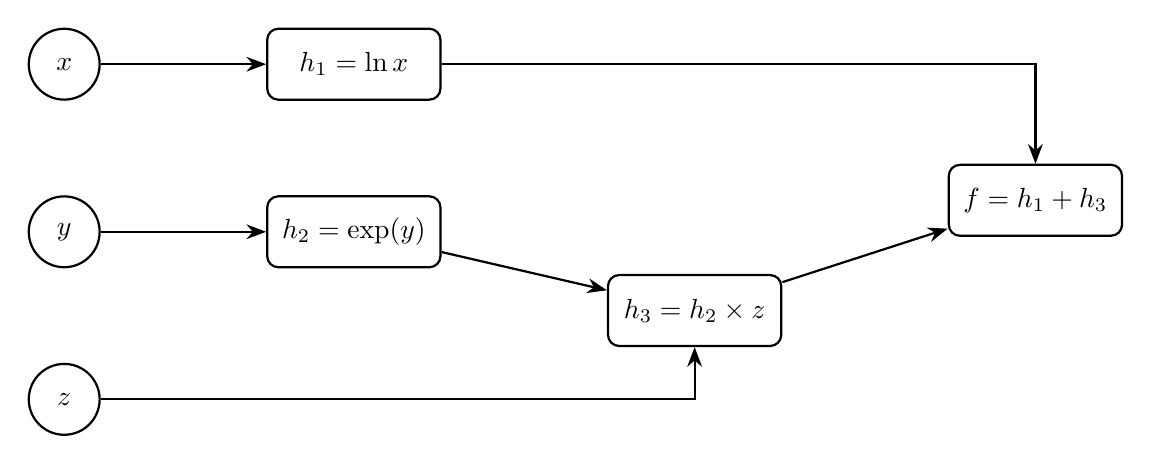
\begin{tikzpicture}[
  node distance=1.2cm and 2.1cm,
  inp/.style={circle,draw,thick,minimum size=9mm},
  op/.style={rectangle,rounded corners,draw,thick,minimum width=22mm,minimum height=9mm,align=center},
  arr/.style={-{Stealth[length=2.5mm]},thick}]
\node[inp] (x) {$x$};
\node[inp,below=of x] (y) {$y$};
\node[inp,below=of y] (z) {$z$};
\node[op,right=of x] (h1) {$h_1 = \ln x$};
\node[op,right=of y] (h2) {$h_2 = \exp(y)$};
\node[op,right=of h2,yshift=-10mm] (h3) {$h_3 = h_2 \times z$};
\node[op,right=of h3,yshift=14mm] (f) {$f = h_1 + h_3$};
\draw[arr] (x) -- (h1);
\draw[arr] (y) -- (h2);
\draw[arr] (h2) -- (h3);
\draw[arr] (z) -| (h3);
\draw[arr] (h1) -| (f);
\draw[arr] (h3) -- (f);
\end{tikzpicture}
\caption{Computation graph. Inputs on the left, output $f$ on the right. Edges carry values forward and gradients backward.}
\end{figure}

\subsection*{5.2 Forward propagation at $[x,y,z] = [1,3,2]$}
\begin{align*}
h_1 &= \ln x = \ln 1 = 0\\
h_2 &= \exp(y) = e^{3} \approx 20.0855\\
h_3 &= h_2\cdot z = e^{3}\cdot 2 = 2e^{3} \approx 40.1711\\
f &= h_1 + h_3 = 0 + 2e^{3} = 2e^{3} \approx 40.1711
\end{align*}

\subsection*{5.3 Backward propagation}
\textbf{Local partial derivatives} (one per edge of the graph), evaluated at $[1,3,2]$ using the forward values from 5.2:
\begin{align*}
\frac{\partial h_1}{\partial x} &= \frac{1}{x} = \frac{1}{1} = 1, &
\frac{\partial h_2}{\partial y} &= e^{y} = e^{3}\approx 20.0855,\\
\frac{\partial h_3}{\partial h_2} &= z = 2, &
\frac{\partial h_3}{\partial z} &= h_2 = e^{3}\approx 20.0855,\\
\frac{\partial f}{\partial h_1} &= 1, &
\frac{\partial f}{\partial h_3} &= 1.
\end{align*}
Every pair not joined by an edge has partial derivative $0$ (for example $\partial h_1/\partial y = 0$ and $\partial h_2/\partial x = 0$).

\textbf{Upstream gradients}, computed from the output back toward the inputs, each one being the gradient arriving at the node times the local derivative of the edge:
\begin{align*}
\frac{\partial f}{\partial f} &= 1\\
\frac{\partial f}{\partial h_3} &= \frac{\partial f}{\partial f}\cdot 1 = 1\\
\frac{\partial f}{\partial h_1} &= \frac{\partial f}{\partial f}\cdot 1 = 1\\
\frac{\partial f}{\partial h_2} &= \frac{\partial f}{\partial h_3}\cdot\frac{\partial h_3}{\partial h_2} = 1\cdot 2 = 2
\end{align*}

\subsection*{5.4 Aggregating with the chain rule}
Each input has a single path to $f$, so each gradient is the product along that path:
\begin{align*}
\frac{\partial f}{\partial x} &= \frac{\partial f}{\partial h_1}\cdot\frac{\partial h_1}{\partial x} = 1\cdot 1 = 1\\
\frac{\partial f}{\partial y} &= \frac{\partial f}{\partial h_3}\cdot\frac{\partial h_3}{\partial h_2}\cdot\frac{\partial h_2}{\partial y} = 1\cdot 2\cdot e^{3} = 2e^{3}\approx 40.1711\\
\frac{\partial f}{\partial z} &= \frac{\partial f}{\partial h_3}\cdot\frac{\partial h_3}{\partial z} = 1\cdot e^{3} = e^{3}\approx 20.0855
\end{align*}
Check against the closed forms $\partial f/\partial x = 1/x$, $\partial f/\partial y = z\,e^{y}$, $\partial f/\partial z = e^{y}$, which give $1$, $2e^{3}$, and $e^{3}$ at $[1,3,2]$. PyTorch autograd returns the same three values ($1.0$, $40.1711$, $20.0855$).

%======================================================================
\section{Programming}

\subsection*{6.1.1 and 6.1.2: Reusing Homework 1 and building the MLP}
The three \texttt{Copy from your HW1} blocks in \texttt{mlp.py} are adapted from my Homework 1 code to this skeleton's contract: \texttt{featurize} averages the GloVe vectors of the in-vocabulary tokens and returns \texttt{None} when there are none, \texttt{create\_tensor\_dataset} drops those reviews and stacks the rest into a float feature tensor and an \texttt{int64} label tensor, and \texttt{accuracy} takes the arg-max over the class dimension. The MLP builds one \texttt{nn.Linear} per consecutive pair in \texttt{[embed\_dim] + hidden\_dims + [num\_classes]}, so an empty \texttt{hidden\_dims} gives the single linear layer of Homework 1, and \texttt{forward} applies the activation after every layer except the last, because \texttt{CrossEntropyLoss} expects raw logits:
\begin{verbatim}
layer_dims = [embed_dim] + list(hidden_dims) + [num_classes]
for in_dim, out_dim in zip(layer_dims[:-1], layer_dims[1:]):
    self.linears.append(nn.Linear(in_dim, out_dim))
...
hidden = inp                                  # (batch_size, embed_dim)
for linear in self.linears[:-1]:
    hidden = self.activation(linear(hidden))  # (batch_size, hidden_dims[i])
logits = self.linears[-1](hidden)             # (batch_size, num_classes)
\end{verbatim}
Before training, the layer shapes were checked for all four configurations, \texttt{forward} was checked against a hand-written composition of the same layers, and \texttt{featurize} and \texttt{accuracy} were checked on small inputs.

\textbf{Setup shared by every run in Section 6.} IMDB, shuffled once with seed 42 (the skeleton's \texttt{shuffle()} was unseeded, and seeding it makes the split reproducible). Dev is the first 1{,}000 training reviews, train the next 20{,}000, and test the first 1{,}000 test reviews. Features are the average \texttt{glove-twitter-50} vector of the NLTK tokens of the lower-cased review. Training uses Adam and cross-entropy for 20 epochs, and the checkpoint with the best dev accuracy is scored on the test set. With 1{,}000 dev reviews, the standard error of an accuracy near 77\% is $\sqrt{0.77\cdot0.23/1000}\approx1.3$ points, which is the scale of the epoch-to-epoch wiggles in every plot below.

\subsection*{6.1.3 Train and evaluate MLPs}
Configurations from \texttt{explore\_mlp\_structures} (sigmoid activation, batch size 64). The template assigns each depth its own learning rate, so depth and step size change together in this experiment.

\begin{center}\small
\begin{tabular}{lccccc}
\toprule
Hidden layers & Learning rate & Dev acc.\ after epoch 0 & Best dev acc. & Min dev loss & Test acc.\\
\midrule
None (linear) & 0.025 & 0.744 & 0.771 & 0.481 & 0.770\\
512 & 0.02 & 0.743 & 0.779 & 0.472 & 0.767\\
512 $\to$ 512 & 0.01 & 0.709 & 0.777 & 0.471 & 0.774\\
512 $\to$ 512 $\to$ 512 & 0.001 & 0.686 & 0.767 & 0.480 & 0.778\\
\bottomrule
\end{tabular}
\end{center}

\begin{figure}[H]
\centering
\begin{subfigure}{0.48\textwidth}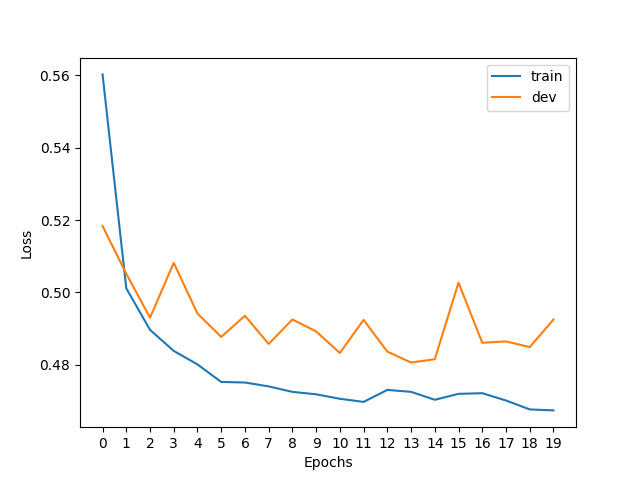
\includegraphics[width=\linewidth]{../hw3/mlp_None_loss.png}\caption{No hidden layer}\end{subfigure}\hfill
\begin{subfigure}{0.48\textwidth}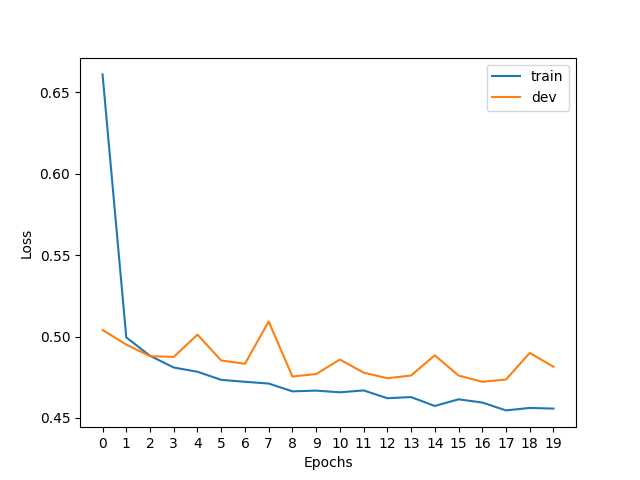
\includegraphics[width=\linewidth]{../hw3/mlp_512_loss.png}\caption{512}\end{subfigure}\\[4pt]
\begin{subfigure}{0.48\textwidth}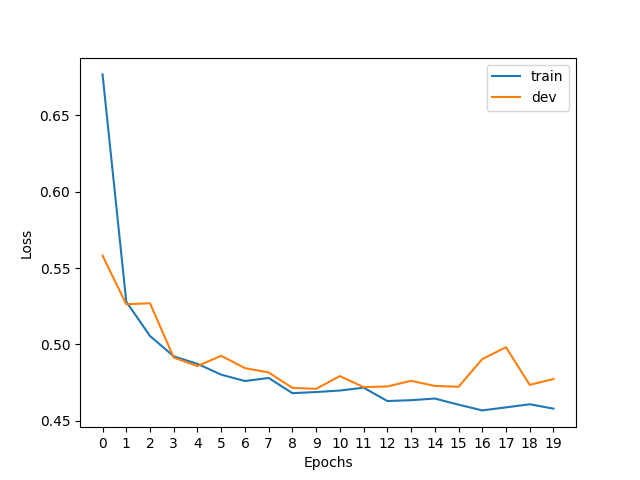
\includegraphics[width=\linewidth]{../hw3/mlp_512-512_loss.png}\caption{512 $\to$ 512}\end{subfigure}\hfill
\begin{subfigure}{0.48\textwidth}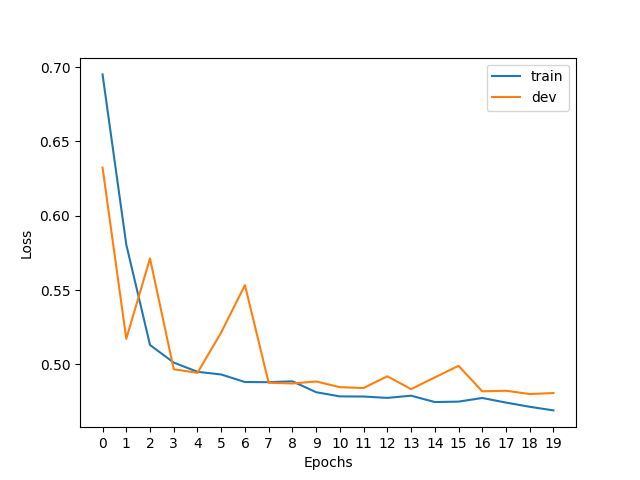
\includegraphics[width=\linewidth]{../hw3/mlp_512-512-512_loss.png}\caption{512 $\to$ 512 $\to$ 512}\end{subfigure}
\caption{Train and dev loss per epoch for each MLP configuration.}
\end{figure}

\begin{figure}[H]
\centering
\begin{subfigure}{0.48\textwidth}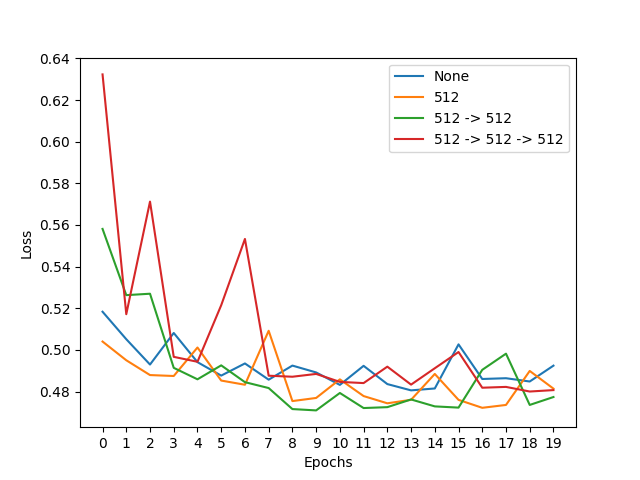
\includegraphics[width=\linewidth]{../hw3/all_mlp_loss.png}\caption{Dev loss}\end{subfigure}\hfill
\begin{subfigure}{0.48\textwidth}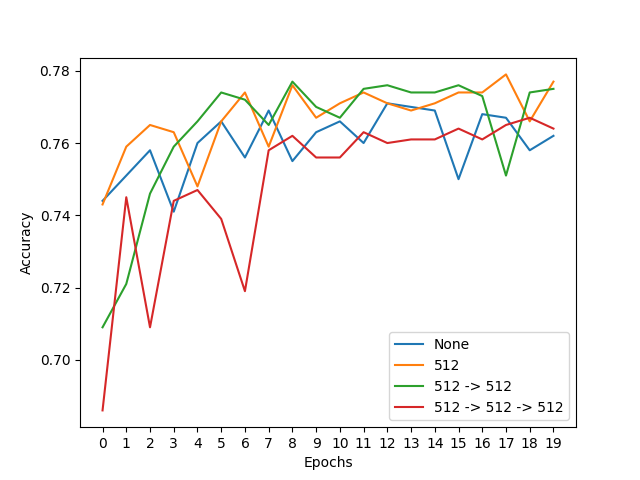
\includegraphics[width=\linewidth]{../hw3/all_mlp_acc.png}\caption{Dev accuracy}\end{subfigure}
\caption{Dev loss and dev accuracy across MLP configurations.}
\end{figure}

\textbf{Findings.} Train loss keeps falling in every configuration while dev loss levels off at 0.47 to 0.49, and the two deeper networks start lower (table) and have bumpier dev curves. Deeper is not better: best dev accuracy is 77.1\%, 77.9\%, 77.7\%, and 76.7\% for zero to three hidden layers, a spread smaller than the noise of a 1{,}000-review dev set. Depth and learning rate change together in this template, so the run cannot separate them, but a likely reason for the flat result is that averaged word vectors discard word order and negation, which leaves extra layers little more information to use.

\subsection*{6.1.4 Embrace non-linearity: the activation functions}
\texttt{SentimentClassifier} takes an \texttt{activation} argument that selects \texttt{nn.Sigmoid}, \texttt{nn.Tanh}, \texttt{nn.ReLU}, \texttt{nn.GELU}, or \texttt{nn.LeakyReLU}, and \texttt{explore\_mlp\_activations} trains one model per activation with everything else fixed (one 512-unit hidden layer, learning rate 0.02, batch size 128, 20 epochs). The Canvas version of the class template does not contain this function, so its fixed hyper-parameters are taken from the upstream JHU CS 601.471/671 hw3 skeleton that this assignment comes from.

\begin{center}\small
\begin{tabular}{lccccc}
\toprule
Activation & Epoch-0 train loss & Best dev accuracy & Min dev loss & Final dev loss & Test accuracy\\
\midrule
Sigmoid & 0.695 & 0.784 & 0.471 & 0.498 & 0.771\\
Tanh & 0.615 & 0.774 & 0.473 & 0.473 & 0.781\\
ReLU & 0.599 & 0.774 & 0.477 & 0.505 & 0.767\\
GELU & 0.602 & 0.787 & 0.472 & 0.519 & 0.760\\
LeakyReLU & 0.570 & 0.778 & 0.464 & 0.464 & 0.774\\
\bottomrule
\end{tabular}
\end{center}

\begin{figure}[H]
\centering
\begin{subfigure}{0.48\textwidth}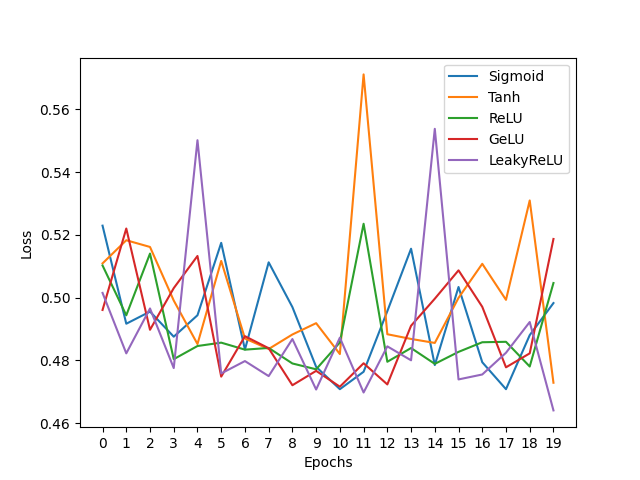
\includegraphics[width=\linewidth]{../hw3/all_mlp_activations_loss.png}\caption{Dev loss}\end{subfigure}\hfill
\begin{subfigure}{0.48\textwidth}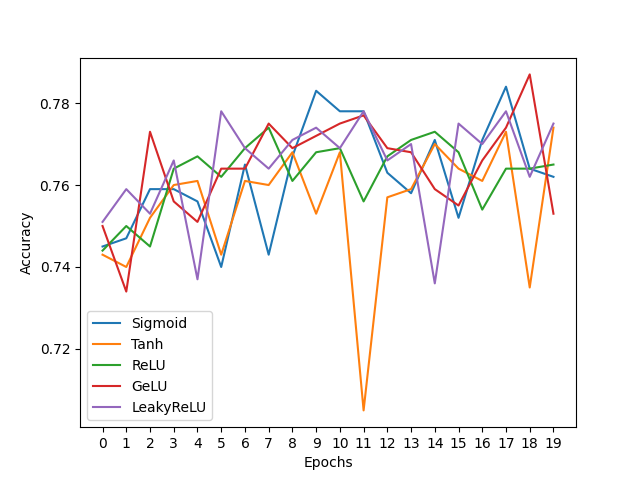
\includegraphics[width=\linewidth]{../hw3/all_mlp_activations_acc.png}\caption{Dev accuracy}\end{subfigure}
\caption{Dev loss and dev accuracy across activation functions (one 512-unit hidden layer).}
\end{figure}

\textbf{Findings.} All five activations end in the same place, with best dev accuracy between 77.4\% and 78.7\% and minimum dev loss between 0.464 and 0.477, differences inside the dev set's noise. Sigmoid starts slowest (average epoch-0 train loss 0.695, about $\ln 2$, against 0.57 to 0.62 for the others), consistent with its smaller slope ($\sigma'\le 1/4$) and its outputs not being zero-centered (Section 3.4), but all five reach 74\% to 75\% dev accuracy by the end of epoch 0. From epoch 5 on, each activation's dev loss moves within a band up to 0.10 wide (tanh), wider than any gap between activations, so keeping the best-dev checkpoint matters more than the choice of activation.

\subsection*{6.1.5 Hyper-parameter tuning: learning rate}
\texttt{explore\_mlp\_learning\_rates} trains the same single 512-unit sigmoid MLP (batch size 64, 20 epochs) at five learning rates: the provided 0.02 plus 0.1, 0.002, 0.0002, and 0.00002 (a factor of 5 above the default, then factors of 10 below it). A separate two-epoch check (\texttt{verification/}\allowbreak\texttt{check\_lr\_saturation.py}) counts how many hidden sigmoid outputs on the dev set are below 0.01 or above 0.99 at learning rates 0.1 and 0.02. It is a separate, seeded run, so its timing differs from the plotted one.

\begin{center}\small
\begin{tabular}{lcccc}
\toprule
Learning rate & Best dev accuracy & Min dev loss & Final dev loss & Test accuracy\\
\midrule
0.1 & 0.772 & 0.482 & 0.528 & 0.776\\
0.02 & 0.780 & 0.470 & 0.480 & 0.772\\
0.002 & 0.769 & 0.479 & 0.482 & 0.779\\
0.0002 & 0.750 & 0.499 & 0.499 & 0.739\\
0.00002 & 0.694 & 0.646 & 0.646 & 0.639\\
\bottomrule
\end{tabular}

\vspace{6pt}
\begin{tabular}{lccc}
\toprule
Saturation check & Epoch & Hidden sigmoid outputs saturated & Dev accuracy\\
\midrule
lr 0.1 & 0 & 100\% & 0.488\\
lr 0.1 & 1 & 99.8\% & 0.738\\
lr 0.02 & 0 & 0\% & 0.750\\
lr 0.02 & 1 & 0.6\% & 0.758\\
\bottomrule
\end{tabular}
\end{center}

\begin{figure}[H]
\centering
\begin{subfigure}{0.48\textwidth}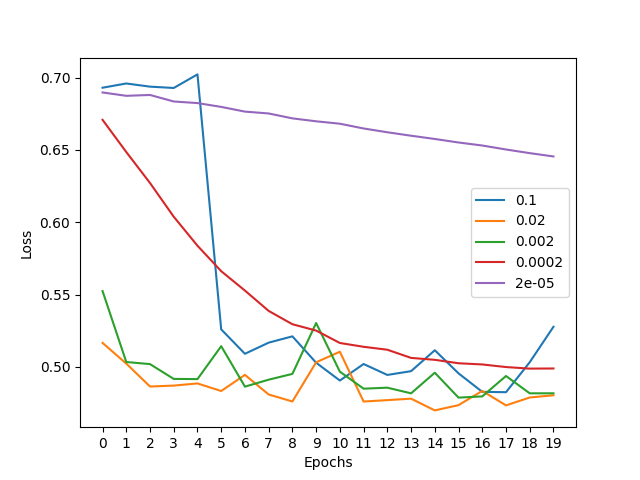
\includegraphics[width=\linewidth]{../hw3/all_mlp_lrs_loss.png}\caption{Dev loss}\end{subfigure}\hfill
\begin{subfigure}{0.48\textwidth}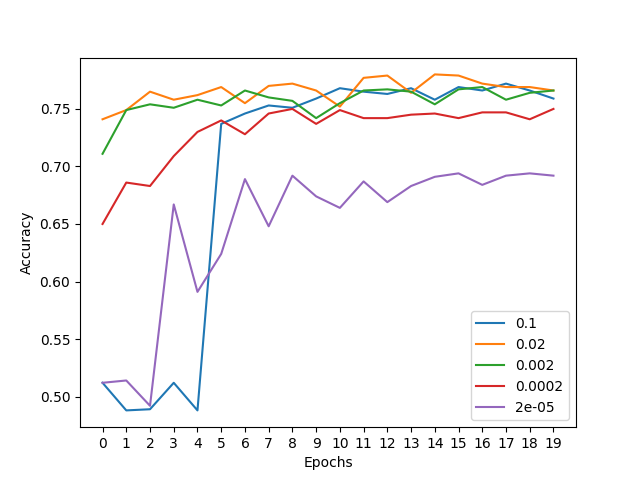
\includegraphics[width=\linewidth]{../hw3/all_mlp_lrs_acc.png}\caption{Dev accuracy}\end{subfigure}
\caption{Dev loss and dev accuracy across learning rates (one 512-unit sigmoid hidden layer).}
\end{figure}

\textbf{Findings.} Learning rates from 0.002 to 0.02 work about equally well (best dev accuracy 76.9\% and 78.0\%), and the provided 0.02 gets there fastest. At the extremes, 0.1 sits at chance for the first five epochs and still reaches 77.2\% at its best, while 0.0002 and 0.00002 improve smoothly but too slowly for 20 epochs and finish at 75.0\% and 69.2\%. The saturation check shows the large steps at 0.1 saturating every hidden sigmoid within one epoch, but accuracy recovered while they stayed saturated, so saturation explains the slow start only in part.


\end{document}
